\documentclass[a4paper,onesided,12pt]{report}
\usepackage{styles/fbe_tez}
\usepackage[utf8x]{inputenc} % To use Unicode (e.g. Turkish) characters
\renewcommand{\labelenumi}{(\roman{enumi})}
\usepackage{amsmath, amsthm, amssymb}
 % Some extra symbols
\usepackage[bottom]{footmisc}
\usepackage{cite}
\usepackage{graphicx}
\usepackage{longtable}
\graphicspath{{figures/}} % Graphics will be here

\usepackage{multirow}
\usepackage{subfigure}
\usepackage{algorithm}
\usepackage{algorithmic}
%\pagestyle{empty}
%\includeonly{introduction} % To only process the given file

\newtheorem{thm}{Theorem}[chapter]
\newtheorem{prop}[thm]{Proposition}
\newtheorem{lem}[thm]{Lemma}
\newtheorem{cor}[thm]{Corollary}
% COVER PAGE
\title{THESIS TITLE}
\turkcebaslik{TEZ BAŞLIĞI}
\degree{B.S., Program Name, Boğaziçi University, 2010}
\author{Selen Parlar}
\program{Your Program}
\subyear{2016}

% APPROVED BY PAGE
\supervisor{Prof. Name Surname}
%\cosuperi{Title and Name of Cosupervisor I}
%\cosuperii{Title and Name of Cosupervisor II}
\examineri{Assoc. Prof. Name Surname}
\examinerii{Assist. Prof. Name Surname}
\examineriii{Name Surname, Ph.D.}
%\examineriv{}
%\examinerv{}
\dateofapproval{DD.MM.YYYY}

\begin{document}

\pagenumbering{roman}
\makemstitle % M.S. thesis
\makeapprovalpage
\begin{acknowledgements}
Acknowledgements come here...
\end{acknowledgements}
\begin{abstract}
One page abstract will come here.  
\end{abstract}
\begin{ozet}
Bir sayfa uzunluğunda özet gelecektir.
\end{ozet}
\tableofcontents
\listoffigures
\listoftables
\begin{symbols}
% The title will be typeset as "LIST OF SYMBOLS".
%
% Use a separate \sym command for each symbols definition.
% First Latin symbols in alphabetical order

\sym{$a_{ij}$}{Description of $a_{ij}$}
\sym{$\mathbf{A}$}{State transition matrix of a hidden Markov model}
% Then Greek symbols in alphabetical order
\sym{}{}
\sym{$\alpha$}{Blending parameter \textit{or} scale}
\sym{$\beta_t(i)$}{Backward variable}
\sym{$\Theta$}{Parameter set}
\sym{ }{}

\end{symbols}

\begin{abbreviations}
 % Abbreviations in alphabetical order
\sym{2D}{Two Dimensional}
\sym{3D}{Three Dimensional}
\sym{AAM}{Active Appearance Model}
\sym{ASM}{Active Shape Model}
\end{abbreviations}


\chapter{INTRODUCTION}
\label{chapter:introduction}
\pagenumbering{arabic}
Start with an introduction...

%\include{experiments_results}
\chapter{EXPERIMENTS AND RESULTS}
\label{chapter:experiments-and-results}

Experiments and results come here... 
\section{Sample Section}
 Always place some text after headings before putting a graphics into
a section as seen in Figure \ref{fig:sample}. 
\begin{figure}[htbp]
\begin{center}
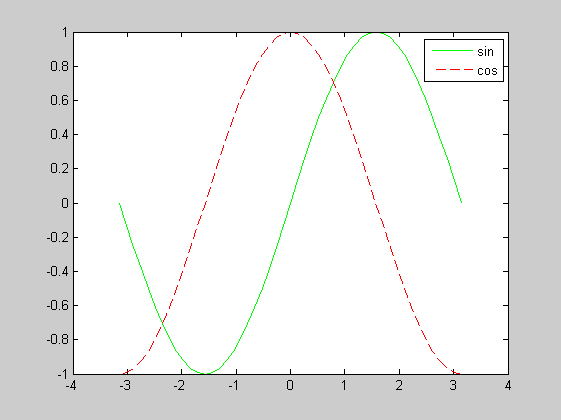
\includegraphics[width=0.5\columnwidth]{sample_figure.png}
\end{center}
\caption{Sin and
Cosine.}
\vskip\baselineskip % Leave a vertical skip below the figure
\label{fig:sample}
\end{figure}

Now, let us cite some studies: one source as \cite{doebelin},  two
sources as \cite{doebelin,exoplanetwebsite} or you may cite three or
more sources as 
\cite{doebelin,exoplanetwebsite,aran2007databaseofnon-manual}.\nocite{
liudissertation} \nocite{paper-IAT-2006-labels}
Observe that they are ordered in the references chapter in the same
order as
they are cited. Let us put a sample table as seen in Table
\ref{table:sample}. Please pay attention that the caption is followed
by a period.

\begin{table}[thbp]
\vskip\baselineskip 
\caption[Sample table]{Sample table.}
\begin{center}
\begin{tabular}{|c|c|c|}\hline
 & \textbf{Header 1}& \textbf{Header 2}\\\hline
\textbf{Row 1} & Bla bla bla& Bla bla bla \\\hline
\textbf{Row 2} & Bla bla bla  & Bla bla bla \\\hline
\end{tabular}
\label{table:sample}
\end{center}
\end{table}



Footnotes should be avoided as possible. If there is an absolute
necessity, footnotes should be used as this.\footnote{Example of a
footnote}

Item lists may be represented as follows:

\begin{itemize}
 \item This is an item. Do not use boldface for the items.
\begin{enumerate}
 \item This is a sub-item. Subsub-items are not allowed.
\end{enumerate}
\item Another item.
\end{itemize}
%  \item 
% \end{enumerate}
Item lists may also be represented as follows:
\begin{enumerate}
 \item This is another enumerated item.
\begin{itemize}
 \item This is another sub-item.
\end{itemize}

\end{enumerate}

\begin{thm}
The solutions of the equation $ax^2+bx+c=0$ with $a\neq 0$ are
$$
x=\frac{-b\pm \sqrt{b^2-4ac}}{2a}
$$
\end{thm}


\begin{proof}
We use the method of completing the square to rewrite $ax^2+bx+c$.
\begin{align*}
ax^2+bx+c&=a\left( x^2 + \frac{b}{a}x+\right)+c \\
  &=a\left( x^2 + \frac{b}{a}x+ \left(\frac{b}{2a}\right)^2
     -\left(\frac{b}{2a}\right)^2 +\right)+c \\
  &=a\left( x+\frac{b}{2a}\right)^2 - 
a\left(\frac{b}{2a}\right)^2+c\\
  &= a\left( x+\frac{b}{2a}\right)^2- \frac{b^2-4ac}{4a}.
\end{align*}
Therefore $ax^2+bx+c=0$ can be rewritten as 
$$
a\left( x+\frac{b}{2a}\right)^2- \frac{b^2-4ac}{4a}=0,
$$
which can in turn  be rearranged as
$$
\left( x+\frac{b}{2a}\right)^2= \frac{b^2-4ac}{4a^2}.
$$
Taking square roots gives
$$
x+\frac{b}{2a}= \frac{\pm \sqrt{b^2-4ac}}{2a}
$$
which implies
$$
x=\frac{-b\pm \sqrt{b^2-4ac}}{2a}
$$
as required.
\end{proof}
Finally, we will put a sample algorithm (PCA algorithm) using the
relevant package in a figure as shown in Figure \ref{alg:pca} and
sample equations.

\begin{figure}[htbp]
\label{alg:pca}
\begin{center}
\framebox[6.0in]{\begin{minipage}[t]{5.9in}
\begin{algorithmic}
\STATE
\STATE \textbf{Require}  $\mathbf{s_i},\ i=1,2,\dots,N$ are normalized
 
\STATE Compute the mean  $\mathbf{\bar{s}}$ using Eq. \ref{eq:mean};
\STATE Form the $N\times2L$ matrix $\mathbf{Q}$ as defined in Eq.
\ref{eq:q};
\IF{ $N < 2\times L$}
\STATE $\mathbf{Q} \Leftarrow \mathbf{Q}^T$ ;
\ENDIF
\STATE Compute the covariance matrix $\mathbf{C}_s$ using Eq.
\ref{eq:cov_matrix};\STATE Decompose $\mathbf{C}_s$
 to its eigenvectors   $\mathbf{e}_k$  and eigenvalues $\lambda_k$
satisfying Eq. \ref{eq:pca};
\IF{ $N < 2\times L$}
\FOR{$k=1$ to $K$}
\STATE $\mathbf{e}_k \Leftarrow \mathbf{Q}\mathbf{e}_k $ ;
\STATE $\mathbf{e}_k \Leftarrow \mathbf{e}_k/||\mathbf{e}_k|| $
(normalization);
\ENDFOR
\ENDIF
\STATE
\end{algorithmic}
\end{minipage}}
\end{center}
\caption[Principal Component Analysis Algorithm]{Principal Component
Analysis Algorithm.}
% \vskip
\end{figure}

\begin{align} 
\mathbf{\bar{s}} & =\frac{1}{N} \sum_{i=1}^N \mathbf{s}_i
\label{eq:mean}   
\\
\mathbf{Q} & =\left[ 
\begin{array}{cccc} 
 \mathbf{s}_1  - \mathbf{\bar{s}} & \mathbf{s}_2 - \mathbf{\bar{s}} &
\cdots & \mathbf{s}_N  - \mathbf{\bar{s}}
\end{array}
\right]_{2L\times N }
\label{eq:q}
\\ 
\mathbf{C}_s & =\frac{1}{N} \mathbf{Q}^T \mathbf{Q}
\label{eq:cov_matrix}
\end{align}

\begin{equation}
    \mathbf{C}_s \mathbf{e}_k = \lambda_k \mathbf{e}_k
    \label{eq:pca}
\end{equation}

\subsection{Example of First Subheadings}
Some text here
\subsubsection{Example of Second Subheadings}
Some text here too.
\chapter{CONCLUSION}
\label{chapter:conclusion}

The conclusions of the thesis should come
here.
% \nocite{NewEntry1,NewEntry2,NewEntry3,NewEntry4,NewEntry5,
% NewEntry6,
% NewEntry7,NewEntry8,NewEntry9,NewEntry10,NewEntry11,NewEntry12}

%\cite{*}
\bibliographystyle{styles/fbe_tez_v11}
\bibliography{references}

\appendix
\chapter{APPLICATION}
The appendices start here.

\end{document}